\chapter{First project} \label{ch:FirstProject}
\chapterquote{Real happiness lies in making others happy.}{Meher Baba}

\graphicspath{{Chapters/FirstProject/Figures/}}
\lstinputpath{Codes-VHDL/Chapter-FirstProject/VHDLCodes/} %path is defined in mypreamble


%\section{Introduction}
In this chapter, UART communication is discussed for NIOS design. Values of Sin(x) is generated using NIOS and the data is  received by computer using UART cable. Since, onchip memory is smaller for storing these values, therefore external memory i.e. SDRAM is used. Further, the received data is stored in a file using `Tera Term' software; finally live-plotting of data is performed using Python.  

In this chapter, we will learn following topics, 
\begin{enumerate}
	\item UART interface,
	\item Receiving the data on computer using UART communication,
	\item SDRAM interface,
	\item Saving data generated by NIOS desgin to a file using `Tera Term',
	\item Updating a existing QSys design and corresponding VHDL and NIOS design,
	\item Live-plotting of data using Python. 
\end{enumerate}

\section{UART interface}
First, create a empty project with name `UartComm' (see Section \ref{sec:new_project}). Next, open the QSys from Tools$\rightarrow$Qsys. Add `Nios Processor', `On-chip RAM (with 20k total-memory-size), `JTAG UART' and `UART (RS-232 Serial Port)' (\textbf{all with default settings}). Note that, Baud rate for UART is set to `115200' (see Fig. \ref{fig:uart_settings}), which will be used while getting the data on computer. Lastly, connect these items as shown in Fig. \ref{fig:uart_qsys_conn}; save it as `Uart\_Qsys.qsys' and finally generate the Qsys system and close the Qsys. Please see Section \ref{sec:CreateGenerateQsys}, if you have problem in generating the QSys system.

\begin{figure}[!h]
	\centering
	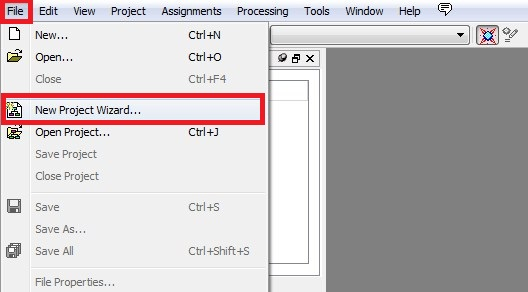
\includegraphics[scale=0.7]{1}
	\caption{UART settings}
	\label{fig:uart_settings}
\end{figure}
 
\begin{figure}[!h]
	\centering
	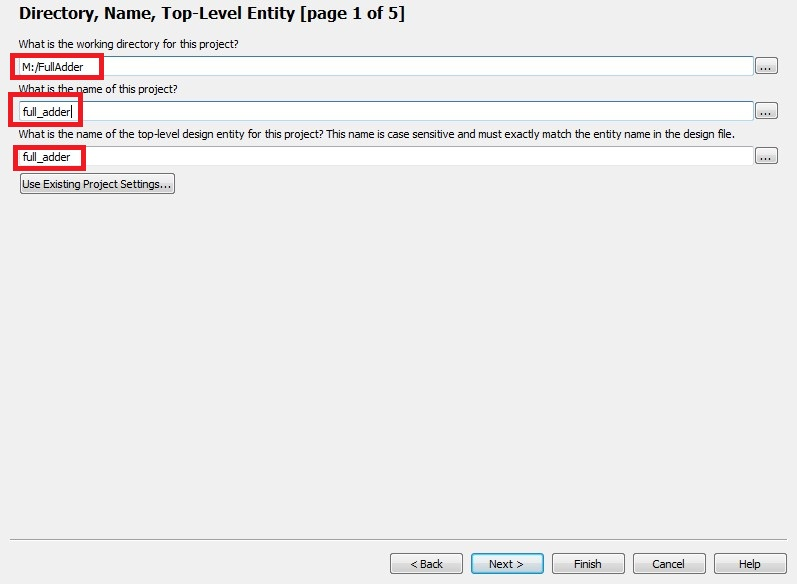
\includegraphics[scale=0.65]{2}
	\caption{Qsys connections}
	\label{fig:uart_qsys_conn}
\end{figure}

Now, add the file `Uart\_Qsys.qip' to the VHDL project. Next, create a new `Block diagram (.bdf) file and import the Qsys design to it and assign correct pin numbers to it, as shown in Fig. \ref{fig:uart_top}. Save it as `Uart\_top.bdf' and set it as `top  level entity'. Lastly, import the pin assignment file and compile the design. Finally, load the design on FPGA board. 

\begin{figure}[!h]
	\centering
	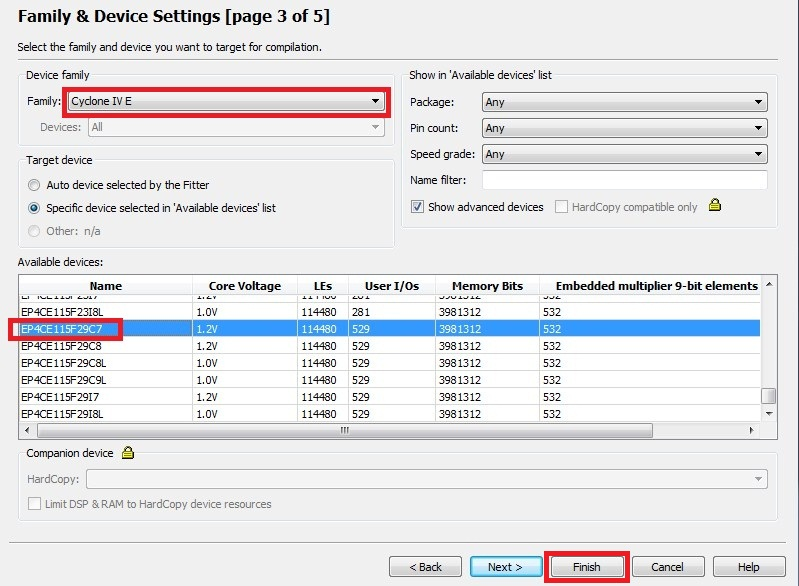
\includegraphics[scale=0.65]{3}
	\caption{Top level entity `Uart\_top.bdf'}
	\label{fig:uart_top}
\end{figure}

\section{NIOS design}
In Chapter \ref{ch:NiosOverview}, we created the `BSP' and `application' file separately for NIOS design. In this chapter, we will use the template provided with NIOS to create the design. For this, open the NIOS software and go to `Files$\rightarrow$New$\rightarrow$NIOS II Application and BSP from Template'. Next, Select the `UART\_Qsys.sopcinfo' file and `Hello World' template and provide the desired name to project e.g. UART\_comm\_app, as shown in Fig , and click `next'. In this window, enter the desired name for BSP file in the `Project name' column e.g. `UART\_comm\_bsp'; and click on Finish.  

\begin{figure}[!h]
	\centering
	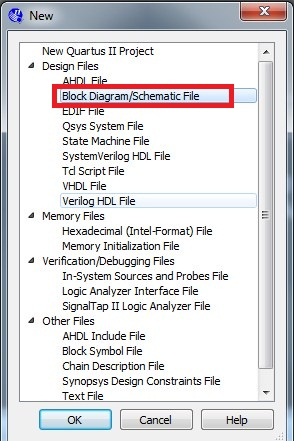
\includegraphics[scale=0.65]{4}
	\caption{Create NIOS project from template}
	\label{fig:nios_name_uart}
\end{figure}

\section{Communication through UART}
To received the data on computer, we need some software like Putty or Tera Term. In this tutorial, we are using `Tera Term software, which can be downloaded freely. Also, we need to change the UART communication settings; so that, we can get messages through UART interface (instead of JTAG-UART)  as shown next. 

Right click on `UART\_comm\_bsp' and go to `NIOS II$\rightarrow$BSP editor'; and select UART\_115200 for various communication as shown in Fig \ref{fig:nios_uart_settings}; and finally click on generate and then click on exit. Now, all the 	`printf' statements will be send to computer via UART port (instead of Jtag-uart). We can change it to JTAG-UART again, by changing UART\_115200 to JTAG-UART again. Note that, when we modify the BSP using BSP-editor, then we need to generate the system again.

\begin{figure}[!h]
	\centering
	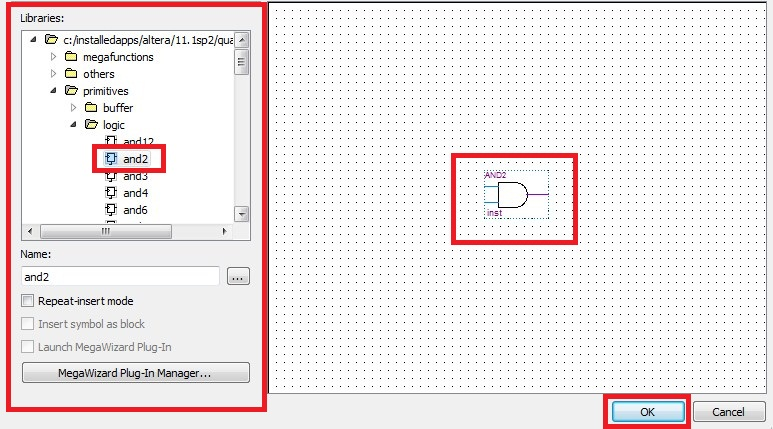
\includegraphics[scale=0.65]{5}
	\caption{UART communication settings in NIOS}
	\label{fig:nios_uart_settings}
\end{figure}

Now, open the Tera Term and select the `Serial' as shown in Fig. \ref{fig:teraTerm}. Then go to `Setup$\rightarrow$Serial Port...' and select the correct baud rate i.e. 115200 and click OK, as shown in Fig. \ref{fig:baudRateteraTerm}. 

\begin{figure}[!h]
	\centering
	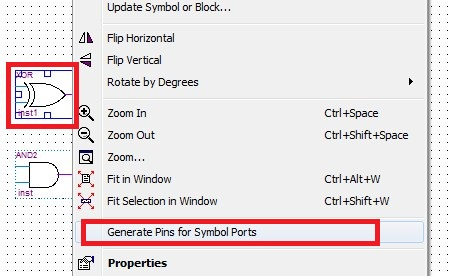
\includegraphics[scale=0.65]{6}
	\caption{Serial communication in Tera Term}
	\label{fig:teraTerm}
\end{figure}

\begin{figure}[!h]
	\centering
	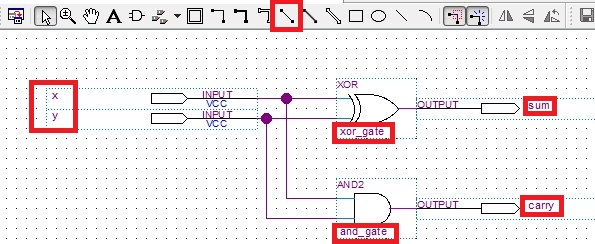
\includegraphics[scale=0.65]{7}
	\caption{Select correct baud rate}
	\label{fig:baudRateteraTerm}
\end{figure}

Finally, right click on `UART\_comm\_app' in NIOS and go to `Run As$\rightarrow$3 NIOS 2 Hardware'. Now, we can see the output on the Tera Term terminal, as shown in Fig. \ref{fig:helloTera}. 

\begin{figure}[!h]
	\centering
	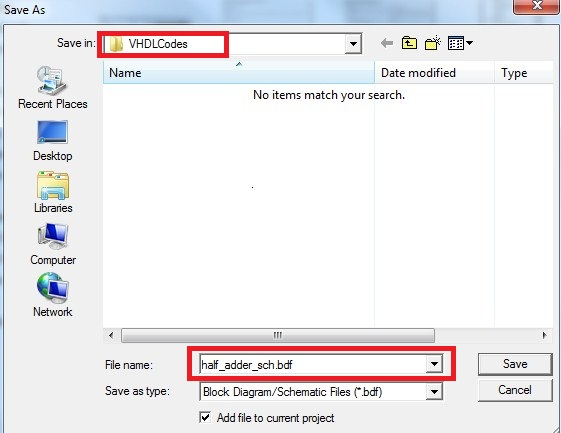
\includegraphics[scale=0.65]{8}
	\caption{`Hello from NIOS II!' on Tera Term}
	\label{fig:helloTera}
\end{figure}

\section{SDRAM Interface}
Our next aim is to generate the Sine waves using NIOS and then plot the waveforms using python. If we write the C-code in current design, then our system will report the memory issue as onchip memory is too small; therefore we need to use external memory. In this section, first, we will update the Qsys design with SDRAM interface, then we will update the Quartus design and finally add the C-code to generate the Sine waves. 

\subsection{Modify QSys}
First, Open the UART\_Qsys.qsys file in QSys software. Now, add SDRAM controller with default settings,  as shown in Fig. \ref{fig:sdram_con}. Next, connect all the ports of SDRMA as shown in Fig. \ref{fig:sdram_connections}. Then, double click the `nios2\_qsys\_0' and select `SDRAM' as reset and exception vector memory, as shown in Fig. \ref{fig:sdram_vector_memory}. 

\begin{figure}[!h]
	\centering
	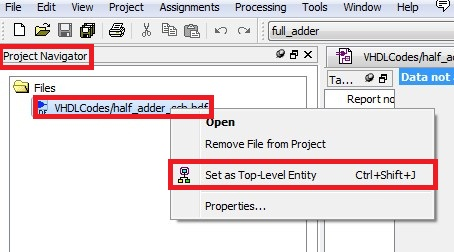
\includegraphics[scale=0.6]{9}
	\caption{SDRAM controller}
	\label{fig:sdram_con}
\end{figure}


\begin{figure}[!h]
	\centering
	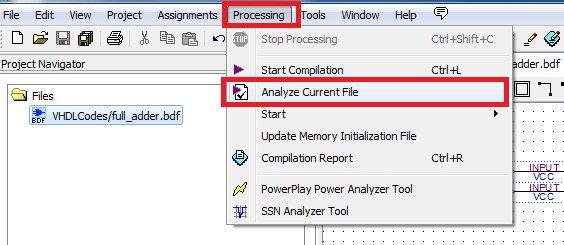
\includegraphics[scale=0.6]{10}
	\caption{SDRAM connections}
	\label{fig:sdram_connections}
\end{figure}


\begin{figure}[!h]
	\centering
	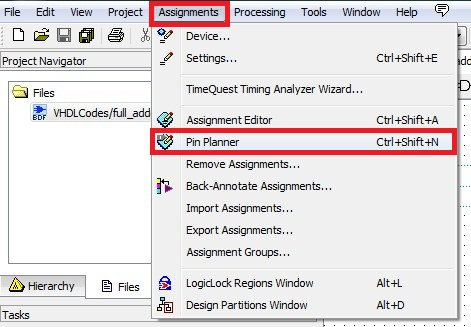
\includegraphics[scale=0.6]{11}
	\caption{Select SDRAM as vector memories}
	\label{fig:sdram_vector_memory}
\end{figure}


Next, we will add `Switches' to control the amplitude of the sine waves. For this add the PIO device of `8 bit with type input', and rename it as `switch', as shown in Fig. \ref{fig:switchForAmplitude} . Finally, go to System$\rightarrow$Assign base addresses, and generate the system. 

\begin{figure}[!h]
	\centering
	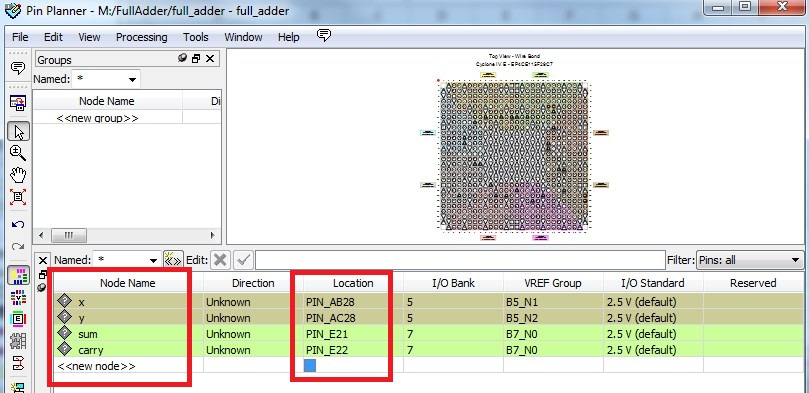
\includegraphics[scale=0.65]{12}
	\caption{Add switches for controlling the amplitude of sine waves}
	\label{fig:switchForAmplitude}
\end{figure}


\subsection{Modify Top level Quartus design}
Now, open the `Uart\_top.bdf' file in Quartus. Right click on the `Uart\_Qsys' block and select `Update symbol or block'; then select the option `Selected symbol(s) or block(s)' and press OK. It will display all the ports for `SDRAM' and switches. Next, we need to assign the correct `pin names' to these ports, as shown in Fig. \ref{fig:SDRAM_Pinassg}.  

\begin{figure}[!h]
	\centering
	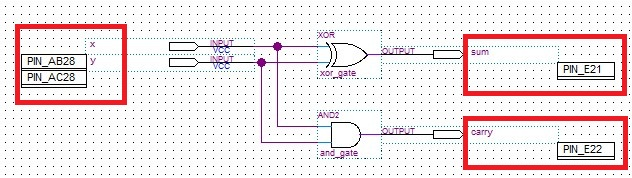
\includegraphics[scale=0.65]{13}
	\caption{Assigning Pins to SDRAM and Switches}
	\label{fig:SDRAM_Pinassg}
\end{figure}

Note that, there should be `-3 ns clock delay' for SDRAM as compare to FPGA clock, therefore we need to add the clock with `-3 ns delay'. For this, double click on the Uart\_top.bdf (anywhere in the file), and select `MegaWizard Plug-In Manager'. Then select `Create a new custom megafunction variation' in the popped-up window and click next. Now, select \textbf{ALTPLL} from \textbf{IO} in \textbf{Installed Plug-Ins} option, as shown in Fig. \ref{fig:dram_clock_altpll}, and click next. Then, follow the figures from Fig. \ref{fig:altpllCreation1} to Fig. \ref{fig:altpllCreation6} to add the ALTPLL to current design i.e. `Uart\_top.bdf'. Finally, connect the ports of this design as shown in Fig. \ref{fig:altpllCreation7}. Note that, in these connections, output of ATLPLL design is connected to `DRAM\_CLK', which is clock-port for DRAM. Lastly, compile and load the design on FPGA board. 

\begin{figure}[!h]
	\centering
	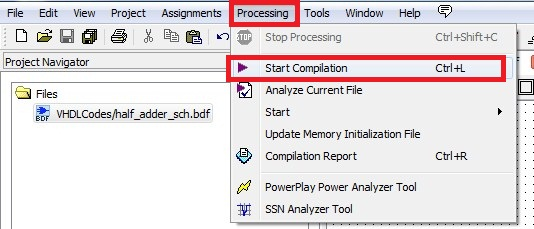
\includegraphics[scale=0.4]{14}
	\caption{ALTPLL generation}
	\label{fig:dram_clock_altpll}
\end{figure}

\begin{figure}[!h]
	\centering
	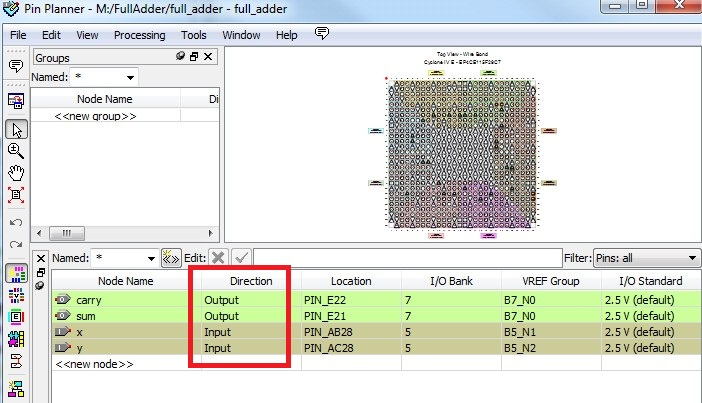
\includegraphics[scale=0.4]{15}
	\caption{ALTPLL creation, step 1}
	\label{fig:altpllCreation1}
\end{figure}

\begin{figure}[!h]
	\centering
	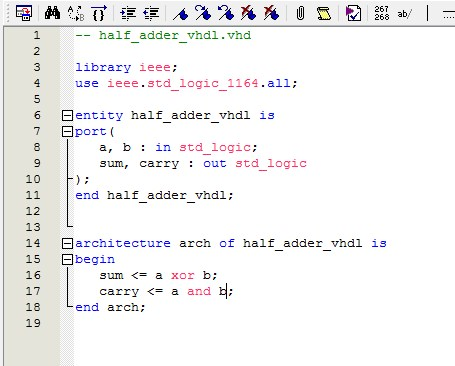
\includegraphics[scale=0.5]{16}
	\caption{ALTPLL creation, step 2}
	\label{fig:altpllCreation2}
\end{figure}

\begin{figure}[!h]
	\centering
	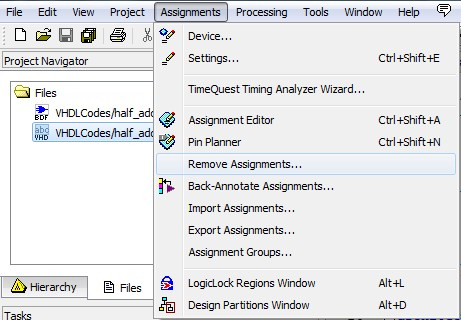
\includegraphics[scale=0.4]{17}
	\caption{ALTPLL creation, step 3}
	\label{fig:altpllCreation3}
\end{figure}

\begin{figure}[!h]
	\centering
	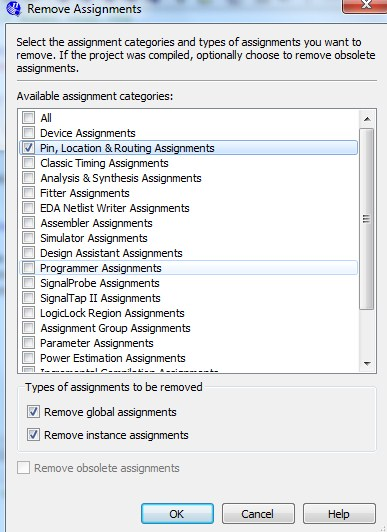
\includegraphics[scale=0.4]{18}
	\caption{ALTPLL creation, step 4}
	\label{fig:altpllCreation4}
\end{figure}

\begin{figure}[!h]
	\centering
	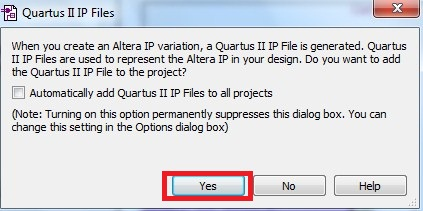
\includegraphics[scale=0.5]{19}
	\caption{ALTPLL creation, step 5}
	\label{fig:altpllCreation5}
\end{figure}

\begin{figure}[!h]
	\centering
	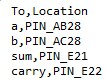
\includegraphics[scale=0.5]{20}
	\caption{ALTPLL creation, step 6}
	\label{fig:altpllCreation6}
\end{figure}

\begin{figure}[!h]
	\centering
	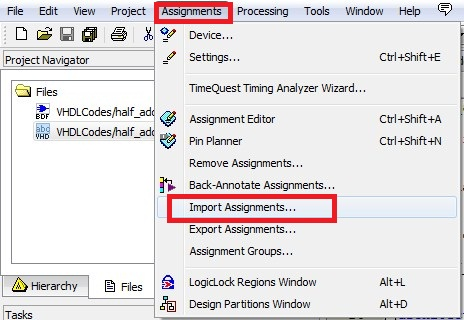
\includegraphics[scale=0.6]{21}
	\caption{Connect ALTPLL design with existing design}
	\label{fig:altpllCreation7}
\end{figure}

\subsection{Updating NIOS design}
Since, we have udpated the QSys design, therefore the corresponding .sopcinfo file is also updated. Further, BSP files depends on the .sopcinfo file, therefore we need to update the BSP as well. For this, right click on `Uart\_comm\_bsp' and go to `NIOS II$\rightarrow$BSP Editor; and update the BSP as shown in Fig. \ref{fig:updateBSPDRAM} and click on `generate' and then click `exit'. Note that, `enable' options are unchecked now, because we are using External memory, which is quite bigger than onchip-memory, so we do not need `small' size options. 

\begin{figure}[!h]
	\centering
	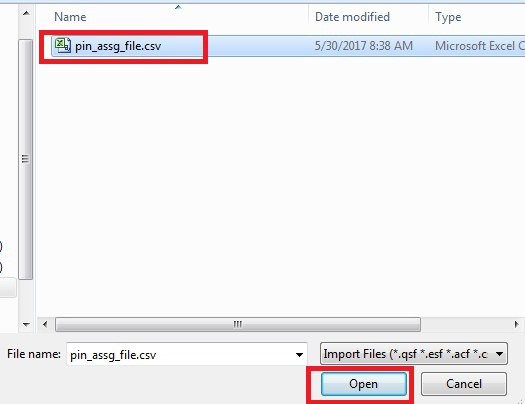
\includegraphics[scale=0.65]{22}
	\caption{Update BSP for new Qsys design}
	\label{fig:updateBSPDRAM}
\end{figure}

Now, update the `hello\_world.c' file as shown in Listing \ref{c:uart_sine_wave}. 

\lstinputlisting[
caption    = {Sin and Cos wave generation},
language = C,
label      = {c:uart_sine_wave}
]{CppCodes/hello_world.c}

In Tera Term, we can save the received values in text file as well. Next, go Files$\rightarrow$Log and select the filename at desired location to save the data e.g. `sineData.txt'. 

Finally, right click on `UART\_comm\_app' in NIOS and go to `Run As$\rightarrow$3 NIOS 2 Hardware'. Now, we can see the decimal values on the screen. If all the switches are at `0' position, then values will be `0.000' as amplitude is zero. Further, we can use any combination of 8 Switches to increase the amplitude of the sine and cosine waves. Also, result will be stored in the  `sineData.txt' file. Content of this file is shown in Fig. \ref{fig:contentLogFile}


\begin{figure}[!h]
	\centering
	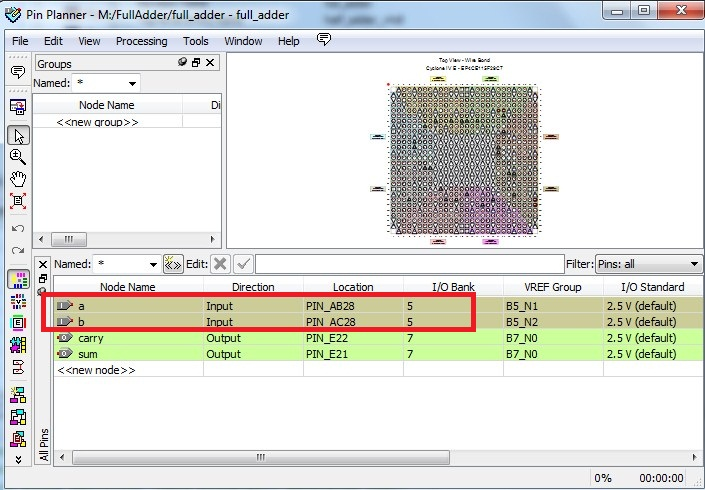
\includegraphics[scale=0.8]{23}
	\caption{Content of `sineData.txt' file}
	\label{fig:contentLogFile}
\end{figure}

\section{Live plotting the data}
In the previous section, we store the sine and cosine wave data on the `sineData.txt' using UART communication. Now, our last task is to plot this data continuously, so that it look line animation. For this save the Listing \ref{pythhon:plotLogData}, in the location where `sineData.txt' is saved. Now, open the command prompt and go to the location of python file. Finally, type \textbf{`python main.py'} and press enter. This will start plotting the waveform continuously based on the data received and stored on the `sineData.txt' file. The corresponding plots are shown in Fig. \ref{fig:plotLogFile}.

\lstinputlisting[
caption    = {Code for live plotting of logged data},
language = Python,
label      = {pythhon:plotLogData}
]{PythonCodes/main.py}

\begin{figure}[!h]
	\centering
	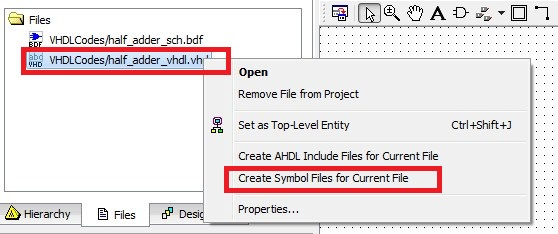
\includegraphics[scale=0.5]{24}
	\caption{Plot of `sineData.txt' file}
	\label{fig:plotLogFile}
\end{figure}


\section{Conclusion}
In this chapter, first we display the `Hello' message using UART and Tera Term. Then, SDRAM is included in the design and correspondingly all the other designs are updated i.e. Quartus and NIOS. Then, the data is stored in the text file and finally it is plotted with the help of Python programming language. 

\section{Introduction}
In this tutorial, full adder is designed with the help of half adders. Here we will learn following methods to create/implement the digital designs using Altera-Quartus software, 

\begin{enumerate}
	\item Digital design using `block schematics',
	\item Digital design using `VHDL codes',
	\item Manual pin assignment for implementation,
	\item Pin assignments using `.csv' file,
	\item Loading the design on FPGA. 
	\item Converting the `VHDL design' to `Symbols'
	\item Converting the `Block schematic' to `VHDL code' and `Symbols'. 
\end{enumerate}

If you do not have the FPGA-board, then skip the last part i.e. `loading the design on FPGA'. Simulation of the designs using `Modelsim' is discussed in Chapter \ref{ch:OverView}. 

\href{https://www.altera.com/downloads/software/quartus-ii-we/111sp2.html}{`Quartus II 11.1sp2 Web Edition'} and \href{https://www.altera.com/downloads/software/modelsim-starter/111.html}{`ModelSim-Altera Starter'} softwares are used for this tutorial, which are freely available and can be downloaded from the \href{https://www.altera.com/downloads/download-center.html}{Altera website}. All the codes can be \href{http://pythondsp.readthedocs.io/en/latest/pythondsp/toc.html}{downloaded from the website}. First line of each listing in the tutorial, is the name of the python file in the downloaded zip-folder. Also, see Appendix \ref{QuartusModelsim} to compile and synthesize the codes of the tutorial.

Note that, Altera-Modelsim-Starter version does not allow simulation of mixed design i.e. VHDL design mixed with Verilog can not be simulated. You need to buy the full edition of Altera-modelsim for this. Further, \href{https://www.aldec.com/en/products/fpga_simulation/active_hdl_student}{`Active-HDL student'} version can be downloaded for free and can be used for mixed-modeling simulation. Lastly, in Active-HDL, all the waveforms can be imported as `.vcd' format (if required); which can be used by Modelsim software as well. To use the .vcd file in Modelsim, first convert it into `.wlf' file. For this, first go to Modelsim's transcript window and then go to the desired directory (which contains the .vcd file) e.g. cd D:/VcdFiles; and then type conversion command i.e. `vcd2wlf VCD\_file\_name.vcd WLF\_file\_name.wlf. This will convert the .vcd file to .wlf file, which can be used in Modelsim to display waveforms.

\section{Creating the project} \label{sec:new_project}
\begin{enumerate}
	\item To create a new project, first open the Quartus and go to File$\rightarrow$New Project Wizard, as shown in Fig. \ref{fig:createNewProject}. 
	
	\begin{figure}[!h]
		\centering
		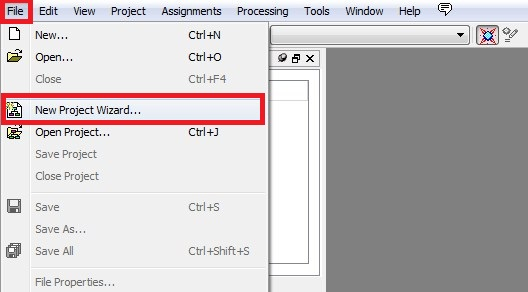
\includegraphics[scale=0.65]{1}
		\caption{Create new project}
		\label{fig:createNewProject}
	\end{figure}
	
	\item `Introduction' window will appear after this, click `next' and fill the project details as shown in Fig. \ref{fig:nameProject}. 
	
	\begin{figure}[!h]
		\centering
		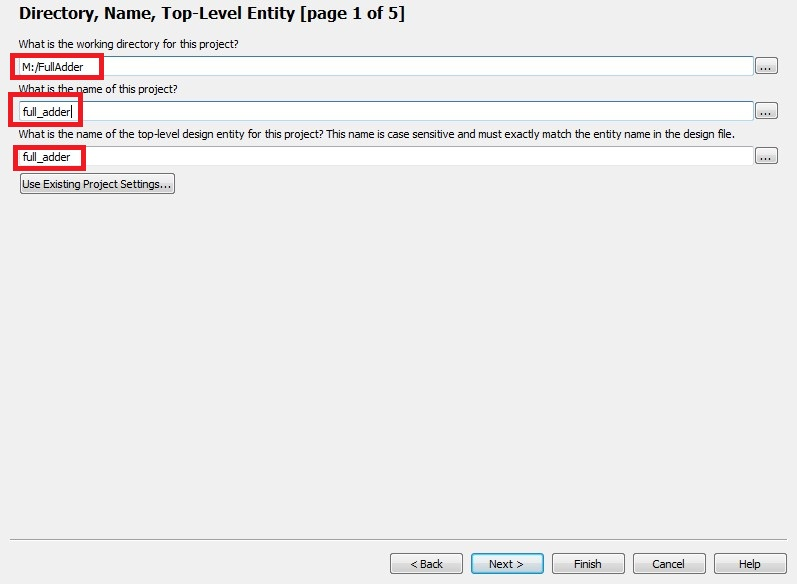
\includegraphics[scale=0.65]{2}
		\caption{Name and location of project}
		\label{fig:nameProject}
	\end{figure}
	
	\item After this, `Add files' window will appear, click on `next' here as we do not have any file to add to this project. 
	
	\item Next, `Family and Device settings' page will appear, select the proper device setting based on your FPGA board and click `Finish' as shown in Fig. \ref{fig:deviceSettings}. If you don't have FPGA board, then simply click `Finish'. 
	\begin{figure}[h]
		\centering
		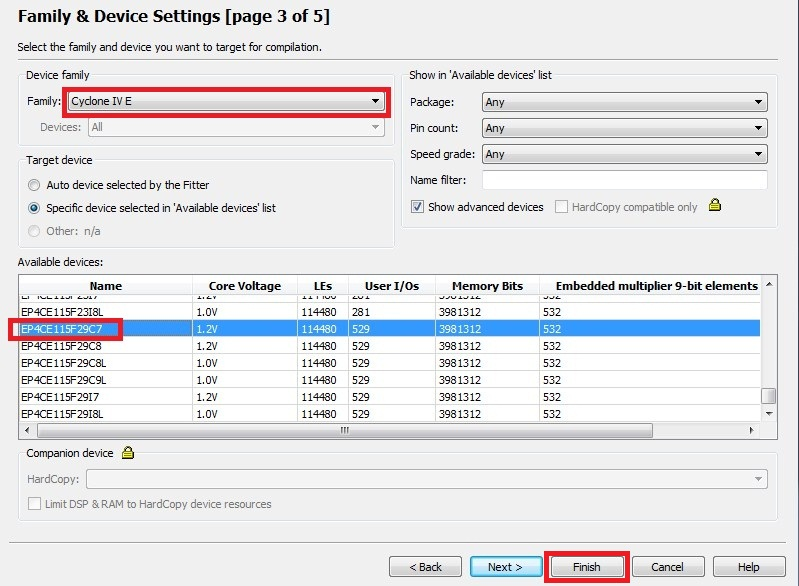
\includegraphics[scale=0.65]{3}
		\caption{Devices settings}
		\label{fig:deviceSettings}
	\end{figure}
	
	
	\item After clicking on finish, the project will be created as shown in Fig. \ref{fig:device_settings}. \textbf{Note that, the tutorials are tested on DE2-115, DE2 (cyclone-II family) or DE0-Nano boards, therefore project settings may be different for different chapters. You need to select the correct device while running the code on your system.} This can be done by double-clicking on the device name, as shown in Fig. \ref{fig:device_settings}.
	
	\begin{figure}[h]
		\centering
		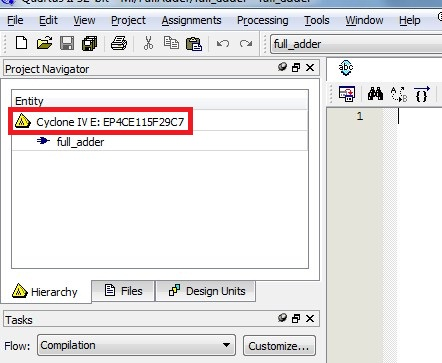
\includegraphics[scale=0.65]{device_settings}
		\caption{Updated Devices settings}
		\label{fig:device_settings}
	\end{figure}
\end{enumerate}

\section{ Digital design using `block schematics'}
Digitals design can be create using two methods i.e. using `block-schematics' and with programming language e.g. VHDL or verilog etc. Both have their own advantages in the design-process, as we will observe in the later chapters of the tutorials. 

In this section, we will create a half\_adder using block-schematics method, as shown below,

\begin{enumerate}
	
	\item For this, click on File$\rightarrow$New$\rightarrow$Block diagram/ Schematics files, as shown in Fig. \ref{fig:block_schematics}; and a blank file will be created.
	
	\begin{figure}
		\centering
		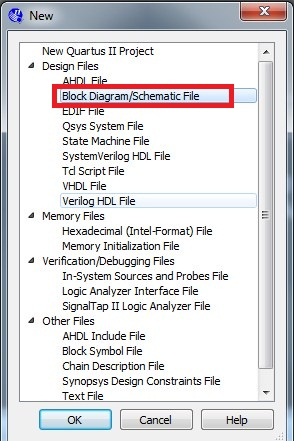
\includegraphics[scale=0.65]{4}
		\caption{Create new block schematics}
		\label{fig:block_schematics}
	\end{figure}
	
	\item Double click (anywhere) in the blank file, and a window will pop-up; select the `and' gate from this window as shown in Fig. \ref{fig:select_gate}. Similarly, select the `xor' gate. 
	
	\begin{figure}
		\centering
		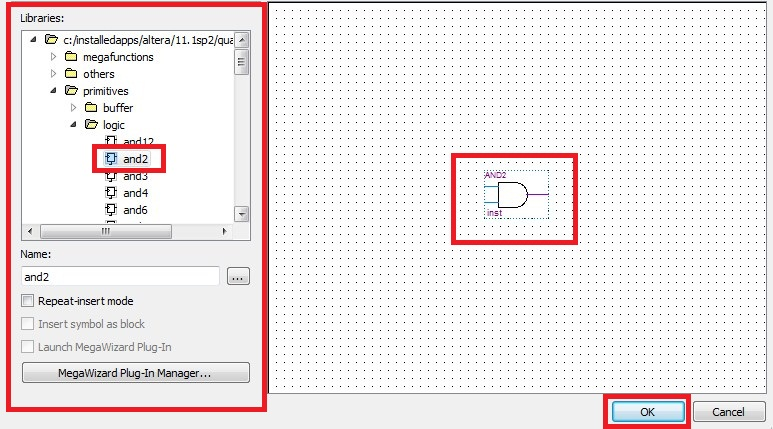
\includegraphics[scale=0.65]{5}
		\caption{Select `and' gate}
		\label{fig:select_gate}
	\end{figure}
	
	\item Next, right click on the `xor' gate and then click on `Generate Pins for Symbol Ports', as shown in Fig. \ref{fig:add_pins}. 
	
	\begin{figure}
		\centering
		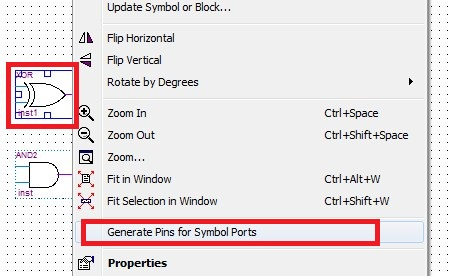
\includegraphics[scale=0.65]{6}
		\caption{Add ports}
		\label{fig:add_pins}
	\end{figure}
	
	\item Now, connect the input ports of `xor' gate with `and' gate (using mouse); then Next, right click on the `and' gate and then click on `Generate Pins for Symbol Ports'. Finally rename the input and output ports (i.e. x, y, sum and carry) as shown in Fig. \ref{fig:make_connections}. 
	
	\begin{figure}
		\centering
		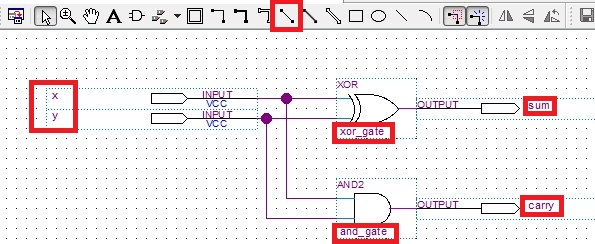
\includegraphics[scale=0.65]{7}
		\caption{Add ports}
		\label{fig:make_connections}
	\end{figure}
	
	\item Finally, save the design with name `half\_adder\_sch.bdf'. It's better to save the design in the separate folder, so that we can distinguish the user-defined and system-generated files, as shown in Fig. \ref{fig:save_project} where VHDL codes are saved inside the `VHDLCodes' folders, which is inside the main project directory. 
	
	\begin{figure}
		\centering
		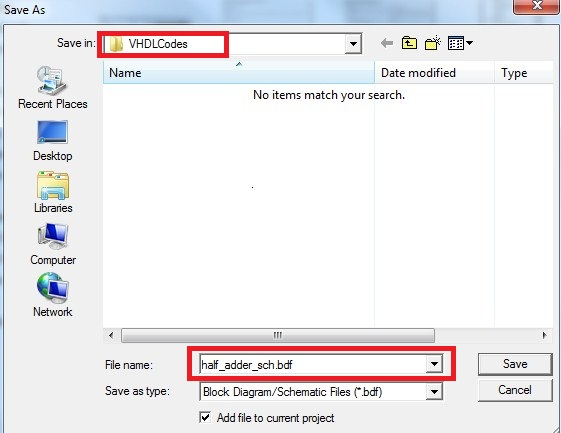
\includegraphics[scale=0.65]{8}
		\caption{Save project in separate directory i.e. VHDLCodes here}
		\label{fig:save_project}
	\end{figure}
	
	\item Since the project name is `full\_adder', where as the half adder's design name is `half\_adder\_sch.bdf' (i.e. not same as the project name), therefore we need to set this design as top level entity for compiling the project. For this, go to project navigator and right click on the `half\_adder\_sch.bdf' and set it as top level entity, as shown in Fig. \ref{fig:top_level_project}.  
	
	\begin{figure}
		\centering
		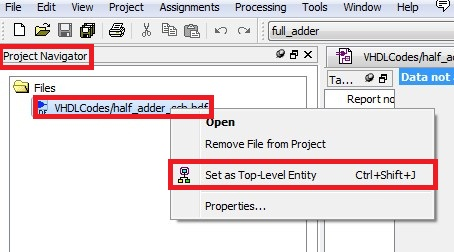
\includegraphics[scale=0.65]{9}
		\caption{Select top level entity for the project}
		\label{fig:top_level_project}
	\end{figure}
	
	\item Now, we can analyze the file as shown in Fig. \ref{fig:analyze_design}. If all the connections are correct that analysis option will not show any error. 
	
	Note that, `start compilation' option (above the Analyse option in the figure) is used when we want to generate the .sof/.pof file, to load the design on the FPGA, whereas analyze option only checks for the syntax errors. We will use `compilation' option in next section. 
	
	\begin{figure}
		\centering
		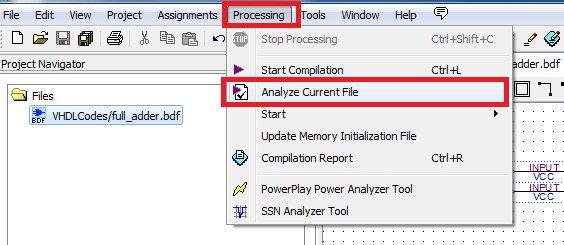
\includegraphics[scale=0.65]{10}
		\caption{Analyze the design}
		\label{fig:analyze_design}
	\end{figure}
	
\end{enumerate}

\section{Manual pin assignment and compilation} \label{sec:compile}\index{pin assignment!manual}
\textbf{Please enter correct pin location according to your FPGA board, as shown in this section. If you do not have the board, then skip this section and go to Section \ref{sec:digital_des_with_vhdl}.}
\\
\\	
Once design is analyzed, then next step is to assign the correct pin location to input and output ports. This can be done manually or using .csv file. In this section, we will assign pin manually. Follow the below steps for pin assignments, 

\begin{enumerate}
	\item First open the `Pin-planner' by clicking Assignments$\rightarrow$Pin Planner as shown in Fig. \ref{fig:pin_planner}.
	
	\begin{figure}
		\centering
		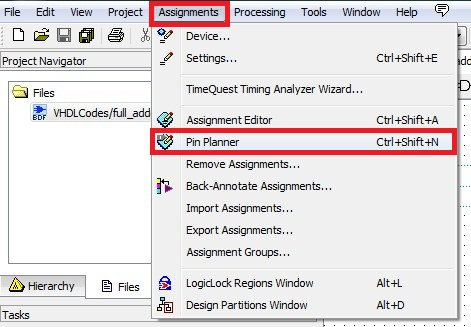
\includegraphics[scale=0.65]{11}
		\caption{Pin planner}
		\label{fig:pin_planner}
	\end{figure}
	
	\item Next, type the names of the input and output ports along with the pin-locations on the board, as shown in Fig. \ref{fig:pin_assgn}. Details of the Pin-locations are provided with the manual of the FPGA-boards e.g. in DE2-115 board, pin `PIN\_AB28' is connected with switch SW0. By assign this pin to `x', we are connecting the port `x' with switch SW0.
	
	\begin{figure}
		\centering
		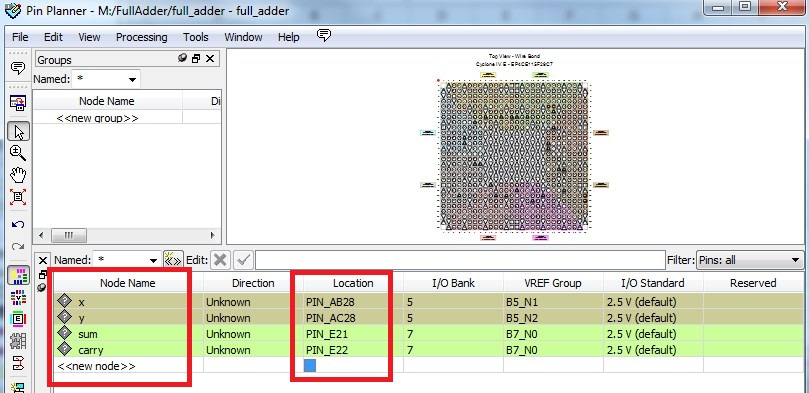
\includegraphics[scale=0.65]{12}
		\caption{Pin assignment}
		\label{fig:pin_assgn}
	\end{figure}
	
	\item After assigning the pin, analyse the design again (see Fig. \ref{fig:analyze_design}). After this, we can see the pin numbers in the `.bdf' file, as shown in Fig. \ref{fig:display_pin_assgn}.
	
	\begin{figure}
		\centering
		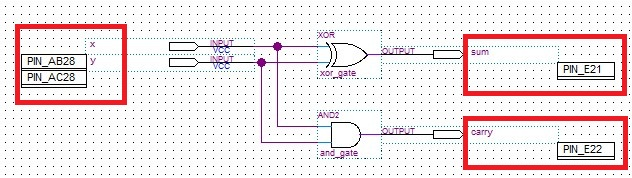
\includegraphics[scale=0.65]{13}
		\caption{Assigned pins to ports}
		\label{fig:display_pin_assgn}
	\end{figure}
	
	\item Finally, compile the design using `ctrl+L' button (or by clicking processing$\rightarrow$Start compilation, as shown in Fig. \ref{fig:start_compilation}). 
	
	\begin{figure}
		\centering
		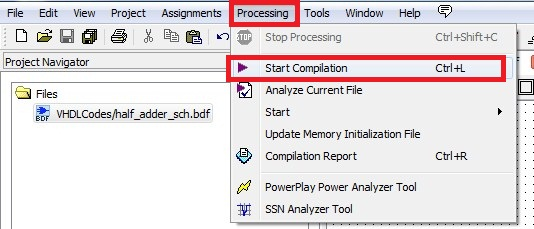
\includegraphics[scale=0.65]{14}
		\caption{Start compilation}
		\label{fig:start_compilation}
	\end{figure}	
	
	\item After successful compilation, if we see the pin-assignment again, then we will find that direction of the pin are assigned now, as shown in Fig. \ref{fig:pin_assgn_direction} (which were set to `unknown' during analysis as in Fig. \ref{fig:pin_assgn})
	
	\begin{figure}[!h]
		\centering
		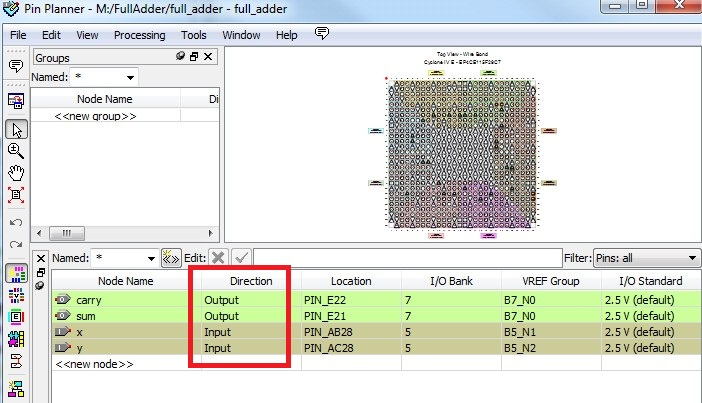
\includegraphics[scale=0.65]{15}
		\caption{Direction of the ports}
		\label{fig:pin_assgn_direction}
	\end{figure}
	
\end{enumerate}

\section{Load the design on FPGA} \label{sec:load_fpga_design}

Follow the below, steps to load the design on FPGA, 

\begin{enumerate}
	\item Connect the FPGA to computer and turn it on. 
	
	\item Full compilation process (Section \ref{sec:compile}), generates the .sof/.pof files, which can be loaded on the FPGA board. To load the design on FPGA board, go to \textbf{Tools$\rightarrow$Programmer}. And a programmer window will pop up. 
	
	\item In the programmer window (see Fig. \ref{fig:load_design}), look for two things i.e. position `1' should display `USB-BLASTER' and position `6' should display the `.sof' file. If any of this mission then follow below steps, 
	
	\begin{itemize}
		\item If USB-BLASTER is missing, then click on `Hardware setup (location 2 in Fig. \ref{fig:load_design})' and then double click on USB-BLASTER in the pop-up window (location 3). This will display the USB-BLASTER at location 4. Finally close the pop-up window. 
		
		\item If `.sof' file is not displayed at location 6, then click on `Add file...' (location 7) and select the `.sof' file from main project directory (or in output\_files folder in main project diretory).
	\end{itemize} 
	
	\item Finally click on the `start' button in Fig. \ref{fig:load_design} and check the operation of `half adder' using switches SW0 and SW1; output will be displayed on green LEDs i.e. LEDG0 and LEDG1. 
	
	\begin{figure}[!h]
		\centering
		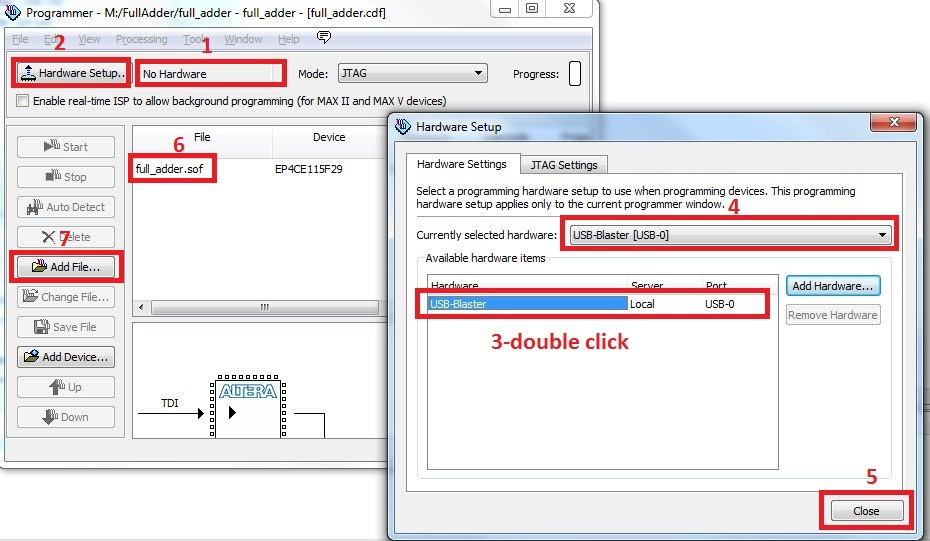
\includegraphics[width=\textwidth]{load_design}
		\caption{Load the design on FPGA}
		\label{fig:load_design}
	\end{figure}
\end{enumerate}

\section{Digital design using `VHDL codes'} \label{sec:digital_des_with_vhdl}

In this section, half adder is implemented using VHDL codes. For this, click on File$\rightarrow$New$\rightarrow$VHDL files, as shown in Fig. \ref{fig:block_schematics}; and a blank file will be created. Type the Listing \ref{vhdl:half_adder_vhdl} in this file and save it as `half\_adder\_vhdl.vhd'. 

\textbf{Now, set this design as `top level entity' (Fig. \ref{fig:top_level_project}).} We can analyze the design now, but we will do it after assigning the pins using .csv file in next section.

\lstinputlisting[
language = Vhdl,
caption    = {VHDL code for half adder},
label      = {vhdl:half_adder_vhdl}
]{half_adder_vhdl.vhd}

\section{Pin assignments using `.csv' file}\index{pin assignment!csv}
In this section, we will learn to assign the pins using .csv files. For this. Note that, we used input port as `a' and `b' in VHDL design (instead of `x' and `y' as in Fig. \ref{fig:make_connections}), so that we can observe the change in the pin assignments. 

To assign the pins using csv file, follow the below steps, 

\begin{enumerate}
	\item First type the content in Fig. \ref{fig:pin_ass_csv} in a text-file and save it as `pin\_assg\_file.csv'. 
	
	\begin{figure}[!h]
		\centering
		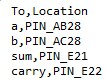
\includegraphics[scale=1]{20}
		\caption{Content of pin\_assg\_file.csv}
		\label{fig:pin_ass_csv}
	\end{figure}
	
	\item Next, click on the Assignments$\rightarrow$Import Assignments as shown in Fig. \ref{fig:import_assg}. And locate the file pin\_assg\_file.csv by clicking on the $\cdots$ button, in the popped-up window, as shown in Fig. \ref{fig:locate_assg}. 
	
	\begin{figure}
		\centering
		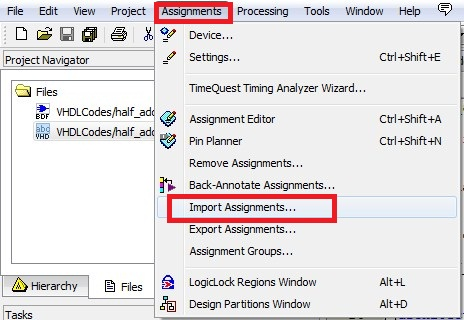
\includegraphics[scale=0.65]{21}
		\caption{Import assignments}
		\label{fig:import_assg}
	\end{figure}
	
	\begin{figure}[!h]
		\centering
		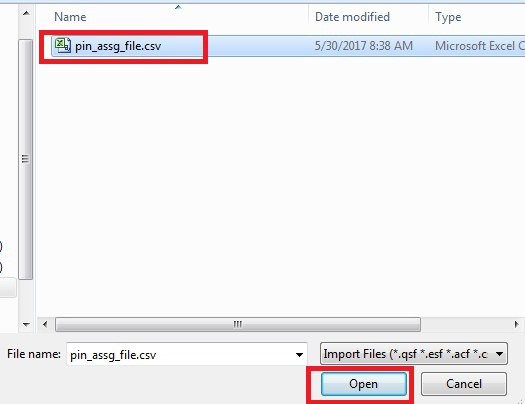
\includegraphics[scale=0.65]{22}
		\caption{Locate the csv file}
		\label{fig:locate_assg}
	\end{figure}
	
	\item Now, analyze the design (Fig. \ref{fig:analyze_design}) and then open the pin planner (Fig. \ref{fig:pin_planner}). We can see the new pin assignments as shown in Fig. \ref{fig:pin_assg_from_csv} (If proper assignments do not happen then check, whether the VHDL design is set as top level or not and import assignments again and analyze the design). 
	
	\begin{figure}
		\centering
		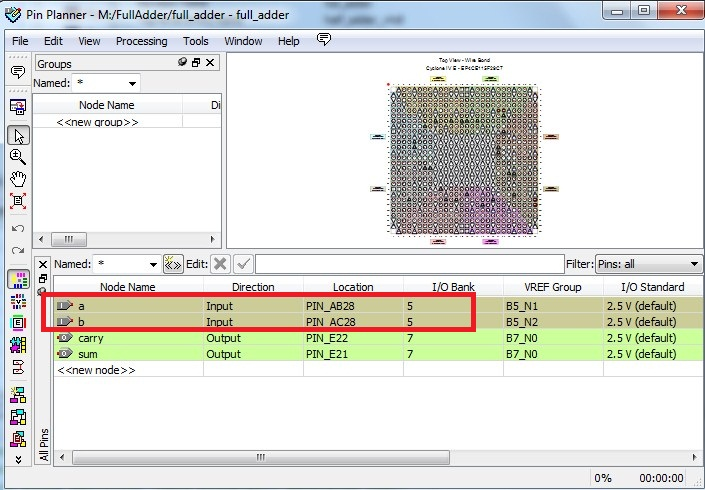
\includegraphics[scale=0.65]{23}
		\caption{Pin assignments from csv file}
		\label{fig:pin_assg_from_csv}
	\end{figure}
	
	\item Finally, compile and load and check the design as discussed in Section \ref{sec:load_fpga_design}. 
\end{enumerate}


\section{Converting the VHDL design to symbol} \label{sec:vhdl_to_symbol}
VHDL code can be converted into block schematic format,  which is quite useful for connecting various modules together. In this section, half adder's vhdl file is converted into schematic and then two half adder is connected to make a full adder. Note that, this connection can be made using VHDL code as well, which is discussed in Chapter \ref{ch:OverView}. 

Follow the below steps to create a full adder using this method,


\begin{enumerate}
	\item Right click on the `half\_adder\_vhdl.vhd' and click on `Create symbol file for current file' as shown in Fig. \ref{fig:vhdl_to_symbol}. It will create a symbol for half adder design. 
	
	\begin{figure}
		\centering
		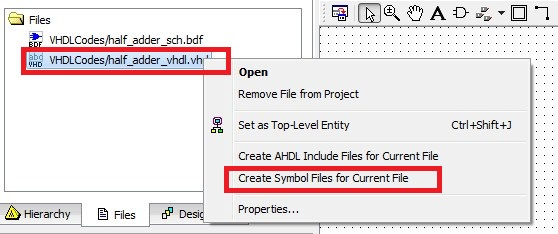
\includegraphics[scale=0.65]{24}
		\caption{Convert VHDL code to symbol}
		\label{fig:vhdl_to_symbol}
	\end{figure}
	%	
	\item Now, create a new `block schematic file' (Fig. \ref{fig:block_schematics}). 
	\item Next, double click on this file and add the half adder symbol as shown in Fig. \ref{fig:ha_symbol}.
	
	\begin{figure}
		\centering
		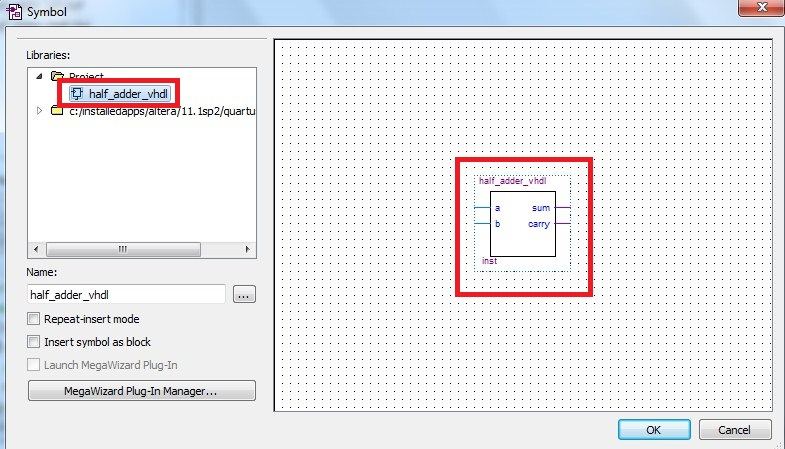
\includegraphics[scale=0.65]{25}
		\caption{Add half adder symbol}
		\label{fig:ha_symbol}
	\end{figure}
	%	
	\item Again add one more `half adder symbol' along with `or' gate and connect these components as shown in Fig. \ref{fig:fa_design}. 
	
	\begin{figure}
		\centering
		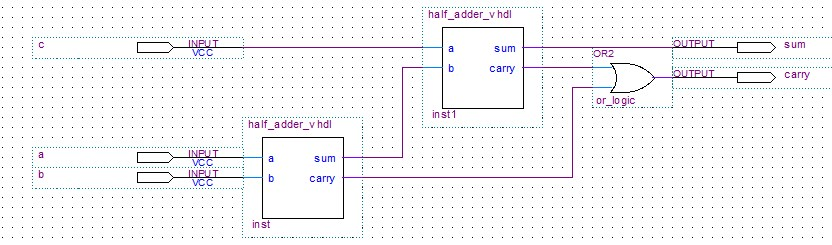
\includegraphics[scale=0.65]{26}
		\caption{Full adder using half adders}
		\label{fig:fa_design}
	\end{figure}
	
	\item Since, one more port (i.e. c) is added to the design, therefore modify the `pin\_assg\_file.csv' as shown in Fig. \ref{fig:update_pin_assg}. 
	
	\begin{figure}
		\centering
		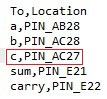
\includegraphics[scale=1]{27}
		\caption{Full adder using half adders}
		\label{fig:update_pin_assg}
	\end{figure}
	%		
	\item Save the design as `full\_adder\_sch.bdf'. 
	\item Import the assignment again; and compile the design (see pin assignments as well for 5 ports i.e. a, b, c, sum and carry). Finally load the design on FGPA. 
\end{enumerate}

\section{Convert Block schematic to `VHDL code' and `Symbol'}

We can convert the `.bdf' file to VHDL code as well. In this section, full adder design is converted to VHDL code. For this open the file `full\_adder\_sch.bdf'. Then go to File$\rightarrow$Create/Update$\rightarrow$Create HDL Design File... as shown in Fig. \ref{fig:bdf_to_vhdl} and select the file type as `VHDL' and press OK; the file will be saved in the VHDLCodes folder (see Fig. \ref{fig:to_vhdl}). The content of the generated `VHDL' file are shown in Listing \ref{vhdl:full_adder_sch}. 

Now, we can convert this VHDL code into symbol as shown in Section \ref{sec:vhdl_to_symbol}. 

\begin{noNumBox}
	Note that, if we can to convert the `.bdf' file into symbol, then we need to convert it into VHDL code first, and then we can convert the VHDL code into symbol file. 
\end{noNumBox}

\begin{figure}[!h]
	\centering
	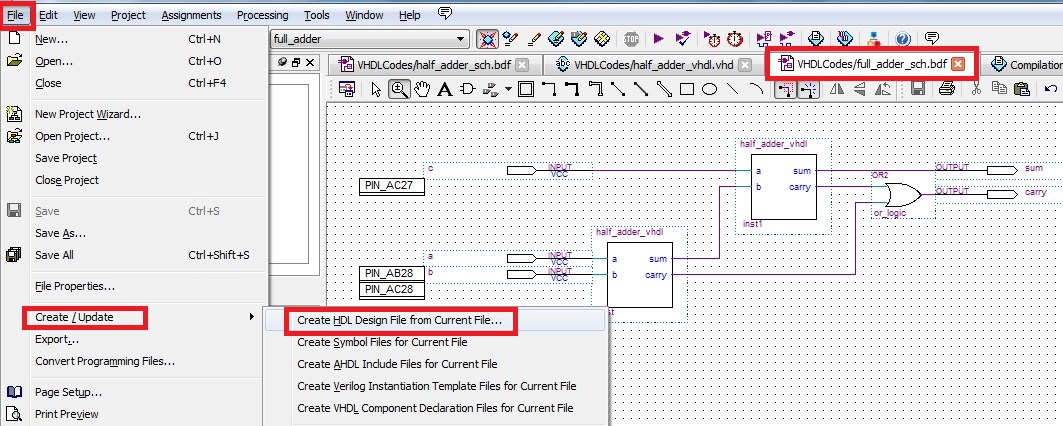
\includegraphics[width=\textwidth]{29}
	\caption{Convert schematic to VHDL}
	\label{fig:bdf_to_vhdl}
\end{figure}


\begin{figure}[!h]
	\centering
	\includegraphics[scale=0.65]{31}
	\caption{Select VHDL}
	\label{fig:to_vhdl}
\end{figure}

\lstinputlisting[
language = Vhdl,
caption    = {VHDL code for full adder},
label      = {vhdl:full_adder_sch}
]{full_adder_sch.vhd}

\section{Conclusion}
In this chapter, we learn to implement the design using schematic and coding methods. Also, we did the pin assignments manually as well as using csv file. Finally, we learn to convert the VHDL code into symbol file; and schematic design into VHDL code. 

\begin{noNumBox}
	Please see the Appendix \ref{NiosQuartusModelsim}  as well, where some more details about symbol connections are shown, along with the methods for using the codes provided in this tutorial. 
\end{noNumBox}
